\documentclass{mcmthesis}
\mcmsetup{CTeX = false,   % 使用 CTeX 套装时,设置为 true
        tcn = 0028, problem = A,
        sheet = true, titleinsheet = true, keywordsinsheet = true,
        titlepage = false, abstract = true}

\usepackage{palatino}
\usepackage{lipsum}
\usepackage{amsmath}  
\usepackage{amssymb}
\usepackage{indentfirst} 



\setlength{\parindent}{1.5em}

\title{The Modeling of Credit Scoring System }

\begin{document}
\begin{abstract}
  
The risk of Internet finance is increasingly apparent. 
It is urgent to build a credit scoring model based on the data of internet finance to improve the risk control level. Based on personal credit history and credit behavior data, credit behavior model derived from data mining and mathematical statistics method can predict individual's future credit performance more accurately, improve the efficiency of Internet operation and reduce the credit cost of Internet financial transaction .
 
We try to construct a credit score model for users by lending information to users and use machine learning model to optimize the performance of credit score based on exploring certain feature engineering.

In feature selection, we employ One-Hot, binning, WOE coding and IV values ​​to extract useful training data from user's data as much as possible.

In the model, we use the basic model of machine learning logistic regression and decision tree for binary training. Performance is less than ideal in logistic regression, although commercial credit ratings are mostly logistic regression. However, under given data conditions, the model is weaker than the decision tree.

With the same characteristics, the decision tree model can achieve better credit score performance. Thus, it can be seen that in the case of weak data, the decision tree may have better performance than logistic regression in modeling credit score. Today's mainstream credit scoring model may have many enhancements without losing the benefits of interpretability.
\begin{keywords}
credit scoring; logistic regression; WOE; IV
\end{keywords}
\end{abstract}
\maketitle
\tableofcontents
\newpage
\section{Introduction}
\subsection{Restatement of Problem}

With the continuous improvement of Internet technology and the increasing number of its users, Internet Finance emerges as the times require. At present, it has been springing up, showing a variety of business models and operation mechanisms. It has advantages which have no for other traditional financial , such as the Internet financial institutions can break through the time and geographical constraints,  provide more efficient financial services for the financing needs of customers on the Internet,  use Internet technology, accelerate business processing speed, and give users a better service experience. But at the same time, risks of Internet financial have raised and become more and more, for example, there are problems such as credit risk and user fraud, there is the urgent need to improve the level of risk control by using the Internet financial data,such as to construct a credit scoring model identification and use the model for effective user level for Internet users.

Credit bureaus can collect the abundant information data by making use of  the Internet, use various data processing methods and data modeling skills, and establish a comprehensive credit evaluation model. At the same time the massive and rich data in the personal credit history and credit behavior based on ones , obtain credit behavior model by using data mining and statistical method,  get more accurately the prediction of the future performance of personal credit, improve the efficiency of operation of the Internet,reduce the cost of credit for the Internet financial transactions ,and be able to estimate the risk of Internet consumer credit. The Internet is an important tool which is irreplaceable in financial institutions . Therefore, the establishment of a precise credit scoring system is of great significance for the Internet financial enterprises. For this problem, the historical business data of a loan institution is given as the original data. The following tasks are completed:
\begin{itemize}
\item it is necessary to extract the main factors that affect the user's credit based on the given data.
\item to contact related macroeconomic data to study the impact of user credit in the macro economic environment.
\item using data mining and other methods, construct the model variables ,  formulate credit rules , establish credit evaluation models , and predict default conditions by models which you make.
\item using the established model to analyze the type of default: the objective type (due to the economic environment or the objective conditions) and the subjective type (the conditions are also deliberately not returned).
\end{itemize}
\subsection{Problem Background}

With the continuous development of Internet technology, its influence has permeated every aspect of life. One of them is that Internet finance emerges as the times require. Compared with the traditional financial, the advantages Internet financial make people favor such as accelerating business processing speed, breaking the time and space constraints, providing faster and more convenient financial services, giving users a better service experience. Neverthless, at the same time, the risks it brings are becoming more and more obvious. For example, there are problems such as credit risk and user fraud. In this context, a set of perfect and effective credit scoring system is becoming particularly important.
\subsection{Our Work}
Credit scoring is using a certain credit score model, which is based on the credit historical data of customers, to get different grades of credit scores. Depending on the customer's credit score, the credit evaluator can analyze the customer's likelihood of repaying on time. Although credit evaluators can also obtain such analysis results by analyzing the credit historical data of customers, use credit scoring make process faster, more objective and more accurate.

Take that Logistic regression algorithm is often used in today's commercial credit scoring models into consideration, we mainly try this algorithm and decision tree algorithm to train. One of the key points of our work is focusing on data cleansing, variable selection and construction of new variables.Some of the major choices for variable selection are based on commonly used credit scores in the industry. For the given data, we mainly do the following thinking:
\begin{itemize}
\item Which of these historical business data is unusable?
\item How to deal with the ``default'' data ratio is not balanced?
\item How to make the model more fully trained on the premise of large amount of data?
\item How to evaluate whether data can promote model training?
\item How to convert some data to make it more suitable for training?
\item How to train the parameters of the algorithm to deal with the adjustment of the problem?
\end{itemize}

\section{Assumptions and Notations}
\subsection{Assumptions}
\begin{itemize}
\item Assume that the historical business data of the lender is stable and trustworthy
\item Assume the default is not affected by emergencies
\item Assume that all borrowers have good credit history before
\end{itemize}

\subsection{Notations}
\begin{table}[htb]
\centering

\begin{tabular}{ll} 
\toprule

Symbol & Specification \\
\toprule
$TP$ & True Positives. \\

$FP$ & False Positives.\\

$FN$ & False Negative. \\

$TN$ & True Negative. \\

$i,j,k$ & Subscripts for various variables. \\

$woe_i$ & A box of evidence weight. \\

$WOE$ & Weight of Evidence .\\

$w$ & Weight. \\

$b$ & Offset or constant. \\

$\mathbf{w}$ & Weight vector. \\

$IV_i$ & Information value of a variable for each group.  \\

$IV$ & Information valu.e \\

$B_i$ & The number of bad customers. \\

$B_T$ & The total of bad customers. \\

$G_i$ & The number of good customers. \\

$G_T$ & The total  of good customers. \\

$TPR$ & The ratio of samples is correctly judged in positive samples.\\

$FPR$ & The ratio of samples is wrongly judged in negative samples.\\

$p_i$ & The probability of the i-th item.\\

$H$ & The uncertainty of measuringrandom variables.\\

$Gini$ & Gini index. \\
\bottomrule
\end{tabular}
\end{table}

\section{Data Processing}
\subsection{Data Screening}
The amount of data is large, so our priority is to filter the data based on its completeness and validity.\\

First, we screen the data of 30,000 historical business data provided by the lender:\\
\begin{itemize}
\item Since tag attributes are crucial and can not be completed, we delete all business data that did not indicate a default.
\item In the analysis of the attributes, we found that there are a large number of missing attributes of AGENT and salary level in the data, in which the salary level can be complemented because it is a numerical attribute with continuous meaning. For AGENT, because it is text type data and Did not find it related to other attributes, so we choose to delete AGENT this attribute.
\end{itemize}

\subsection{Data Merging}
\begin{itemize}
\item When processing the data we found that the education level variables, there are college and below, junior high school and junior high school, the four classification of repeated phenomena, which are repeated graduate, doctoral and master's degree and more than three kinds of classification, so we will and specialist and below master degree or above and two classification.
\item At the same time, we found that two kinds of definitions of divorce and divorce were duplicated in the marital status. We merged them into divorce. At the same time, we considered the semantic description of marital status. We merged the widowhood into divorce and merged the other into the unmarried.
\item For borrowing time, we provide data from January to June 2017, so we combine it into 6 categories representing 6 months to facilitate later use. .
\item For the working provinces, we divide the provinces into four large areas, the eastern, the northeast, the central and the western regions, according to the division of the sixteen regions of the Communist Party of China and the development of the provinces in the past year (Figure).
\end{itemize}

\begin{figure}[h]
\large
\centering
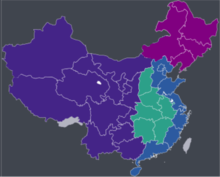
\includegraphics{map.png}
\caption{National Economic Zone} \label{fig:National Economic Zone}
\end{figure}

\subsection{Missing Value Processing}

In statistics, missing data occur when no data value is stored for the variable in an observation.Missing data are a common occurrence and can have a significant effect on the conclusions that can be drawn from the data.

In the data we use, there is a large amount of data that is missing a salary grade variable, and we consider doing so due to the lack of a large amount of data and the variable is a numeric data with a continuous relationship. We have statistics on the available data and found that the overall data is normally distributed.
\newpage
\begin{figure}[h]
\small
\centering
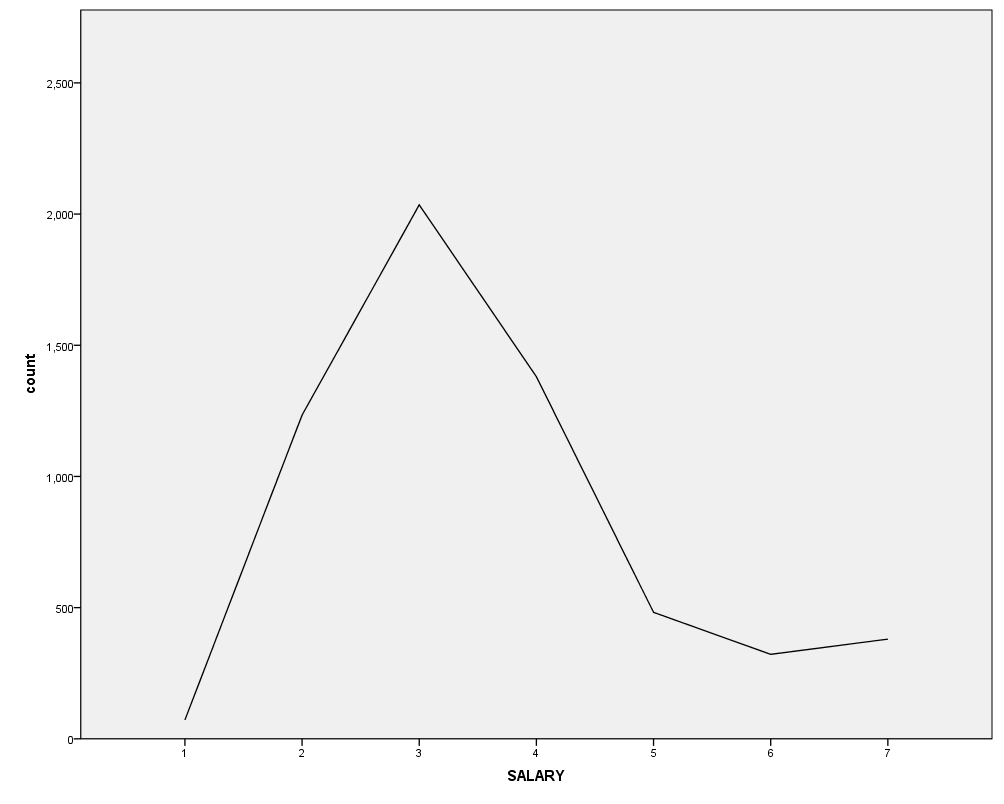
\includegraphics[width=10cm]{sosl.png}
\caption{The level of salary statistics} \label{fig:The level of salary statistics}
\end{figure}

Then we consider that the pay scale may be influenced by the level of education and the work area, so we will analyze it on the assumption that different education levels and pay scales are different from those in the work area.

\begin{figure}[h]
\small
\centering
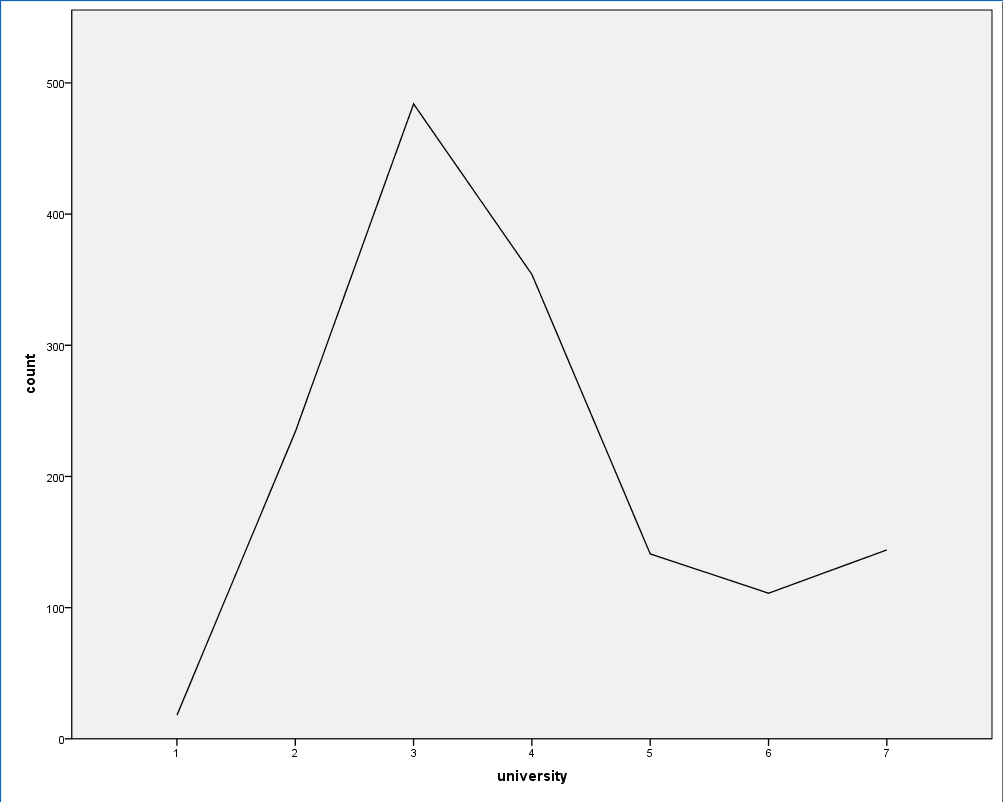
\includegraphics[width=10cm]{un.png}
\caption{Undergraduate education level of the amount of salary level statistics} \label{fig:Undergraduate education level of the amount of salary level statistics}
\end{figure}

We found that at different levels of education, salary levels are basically normal distribution, so taking the level of compensation at different levels of education found. The proportion of high salaries at the educational level of masters and above is higher than that of other education levels. However, taking into consideration the low level of data in this level of education, The horizontal approximation is seen as a normal distribution.
\newpage

\begin{figure}[h]
\small
\centering
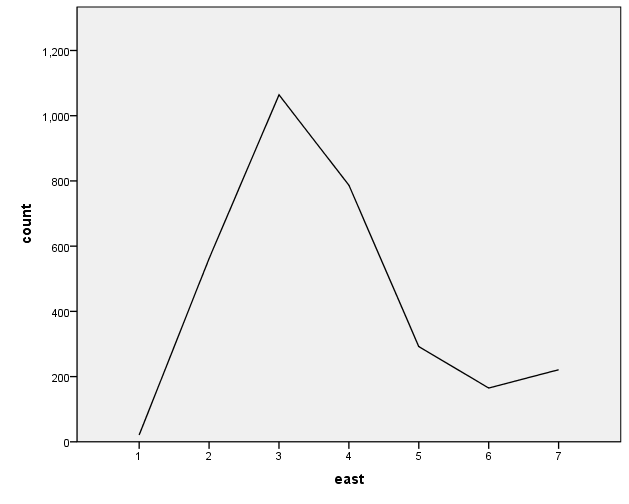
\includegraphics[width=10cm]{east.png}
\caption{The eastern region of the amount of salary level statistics} \label{fig:The eastern region of the amount of salary level statistics}
\end{figure}

For different workplaces, we also analyze their salary levels.

We also found that in all workplaces, all salary levels are normally distributed, so we conclude that the salary level in this data is normally distributed, with no educational level or work area impact.

In this regard, we take the average and mode and draw the relevant charts for a preliminary analysis.

\begin{figure}[h]
\small
\centering
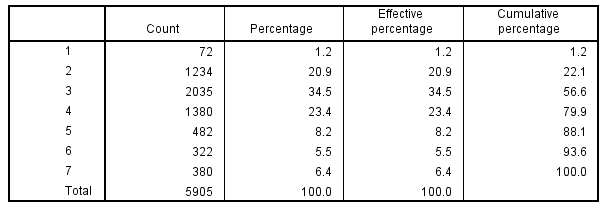
\includegraphics[width=12cm]{sp.png}
\caption{The amount of salary level statistics} \label{fig:The amount of salary level statistics}
\end{figure}

We can see that the average is 3.58 and the mode is 3. Taking into consideration and facilitating our later use, we decided to set the missing value of all pay levels to 3.

\subsection{Unbalanced Data Processing}
Statistical statistics on the number of data labels found that the number of non-defaults is much larger than the number of defaults (as shown in the figure), which easily leads our model to predict all the results as non-defaulting during training, and the final correctness rate is as high as 0.9 on the surface The actual prediction accuracy of the default is 0, in order to avoid this phenomenon, we under-sampled and oversampled the data processing, making the difference between the two types of data should not be too large
\newline
\begin{figure}[h]
\small
\centering
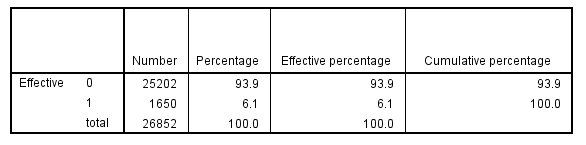
\includegraphics{ttns.png}
\caption{Tag type number statistics} \label{fig:Tag type number statistics}
\end{figure}

\section{Our Model}
Considering the current credit scoring model and the industry's interpretative requirements for the credit scoring model, we considered is logistic regression algorithm as the initial strategy based on available information.

For the strategy we adopted, the marital status, if expressed in a simple order, would make some of them considered similar, but that was not the case.Because the attribute of marriage itself is not sequential, so we code it One-Hot.In a similar way, we do the same to the data of education background

Finally we take the province data into consideration, the data we use reflect the regional is a 6-digit code. It is observed that the left-most 2-digit of the 6-digit code  represents province. Hence we keep the left-most 2-digit. As we all know, China is a big country with many provinces. Aftering reviewing the relevant information, we find that China can be divided into four major economic regions: the eastern region, the northeast region, the central region and the western region.The main contents of economic and social development in various regions are: development in the west, rejuvenation in the northeast, rise in the middle and development in the east. Taking into account the loan, credit score link with economy, we divided the provinces data according the four regions:
\begin{itemize}
  \item Northeast: Heilongjiang, Jilin, Liaoning, Hulunbeier, Xing'an League, Tongliao, Chifeng, Xilin Gol League in eastern Inner Mongolia Autonomous Region
  \item Middle: Shanxi, Henan, Hubei, Hunan, Jiangxi, Anhui
  \item East: Beijing, Tianjin, Hebei, Shandong, Jiangsu, Shanghai, Zhejiang, Fujian, Guangdong, Hainan 
  \item West: Sichuan Province, Guangxi Zhuang Autonomous Region, Guizhou Province, Yunnan Province, Chongqing Municipality, Shaanxi Province, Gansu Province, West Inner Mongolia Autonomous Region, Ningxia Hui Autonomous Region, Xinjiang Uygur Autonomous Region, Qinghai Province and Tibet Autonomous Region
\end{itemize}

The following is based on the left-most 2-digit of the ID card number:

\begin{itemize}
  \item Northeast: 21,22,23
  \item Middle: 14,41,42,43,36,34
  \item East: 11,12,13,37,32,31,33,35,44,46  
  \item West: 51,45,52,53,50,61,62,15,64,65,63,54
\end{itemize}

In fact, there is no order between provinces, so we code the data of province One-Hot once again.
\newline
\\

After the above steps, the current data should be able to train. However, before training, we still need to do some feature Engineering.We use a method commonly used in the industry for screening based on IV.The full name of IV is Information Value, we should get the woe of the data before getting IV of the data.

WOE (weight of Evidence) reflects an influence on the proportion of default when an independent variable takes a certain value. After WOE encoding, the independent variable actually has some standardized nature, that is, each value of the independent variable van be directly compared (between WOE), and various values between different independent variables can also be directly compared by WOE. Furthermore, we can study the variation (fluctuation) of the WOE in the independent variable to construct the contribution rate and relative importance of each independent variable in combination with the coefficients fitted by the model.In general, the greater the coefficient, the greater the variance of woe, the greater the contribution of the independent variable (similar to some variance contribution), which can be intuitively understood.

To sum up, the process of independent variables (including coding and filtering) is largely based on the evaluation of the effects of univariate models when doing credit scoring models. In this evaluation process, ROC and IV examine the impact of independent variables on the target variables from different perspectives. Based on this investigation, we use  WOE to encode non-numeric relational variables so that we can more intuitively understand the effect and direction of the independent variables on the target variables and improve the prediction results.

First, group the variable into groups.And then, for each group , for the i-th group:
\[woe_i = \ln(\frac{B_i / B_T}{G_i / G_T})\eqno (1)\]

For example, if only the absolute value of woe is summed. Assuming that some groups such as Group A and Group B. Group A is with small number, which is opposite to Group B (obviously such a group is not reasonable), then woe of group B is very small which is opposite to Group A. The outcome of the case is that the sum of woe will not be small, but apparently so unreasonable.
\[IV_i = (\frac{B_i}{B_T} - \frac{G_i}{G_T}) * woe_i\eqno (2)\]
\[IV = \sum_{k=0}^n IV_i\eqno (3)\]

Finally, we can sort the variables according to the IV size of each variable. The larger IV, the more variables to be retained.

\begin{table}[h]
\centering
\caption{Predicted based on IV value}
\begin{tabular}{|c|c|}
\hline
IV & Predictive Ability\\
\hline
<0.03 & NAUGHT\\
\hline
0.03 - 0.09 & LOW\\
\hline
0.1 - 0.29 & MIDDLE\\
\hline
0.3 - 0.49 & HIGH\\
\hline
>= 0.5 & VERY HIGH\\
\hline
\end{tabular}
\label{tab1}
\end{table}

Take the credit scorecard modeling scenario as an example: X is the customer sample field, Y indicates whether the customer is overdue, where Y = 1 means overdue, Y = 0 means not overdue. We want to be able to use the information known to our clients to predict the probability of overdue after the customer borrows, in order to decide whether to lend.

\begin{table}[h]
\centering
\caption{IV of the Attribute}
\begin{tabular}{|c|c|}
\hline
Attribute & IV\\
\hline
LOAN\_DATE & 0.112\\
\hline
IS\_LOCAL & 0.032\\
\hline
WORK\_PROVINCE' & 0.233\\
\hline
EDU\_LEVEL & 0.025\\
\hline
MARRY\_STATUS & 0.012\\
\hline
SALARY\_LEVEL & 0.173\\
\hline
HAS\_FUND & 0.000\\
\hline
\end{tabular}
\label{tab2}
\end{table}

We calculate the WOE of each attribute field for the previous data, and then calculate the corresponding IV based on the WOE . IV measures the amount of information on a variable which explain the reason IV can be used to represent the predictive power of a variable.
\section{Analysis of the Result}
Through the prediction of the test data, the accuracy rate is 0.74, the recall rate is 0.51, and the overall prediction accuracy rate is 0.62 (see picture). Overall, the effect is not good. However, the issue of default assessment with credit rating, the more emphasis on recall rate, so the recall rate of 0.51 basically meet the demand.
\newpage
\begin{figure}[h]
\small
\centering
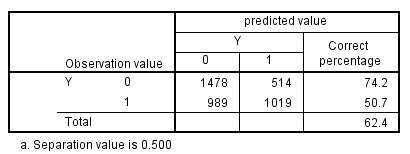
\includegraphics[width=12cm]{result.png}
\caption{result analysis} \label{fig:result analysis}
\end{figure}

Draw its ROC curve can be seen that the model can easily predict whether the default. However, in the process of model establishment, the model can only detect the correctness of the model to a certain extent because the quantity is less than the real one.
\begin{figure}[h]
\small
\centering
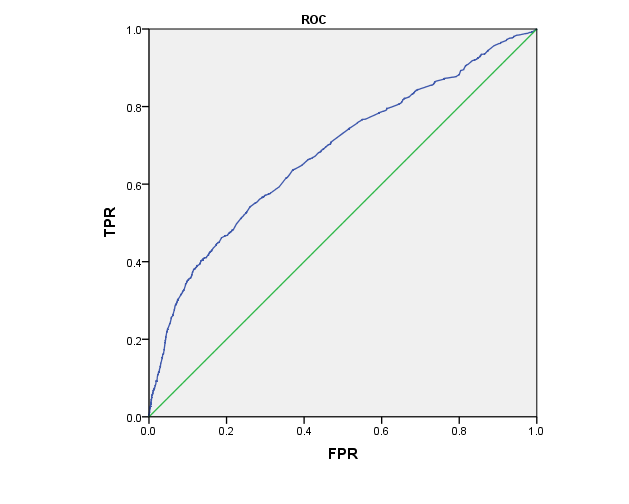
\includegraphics[width=12cm]{ROC.png}
\caption{ROC} \label{fig:ROC}
\end{figure}

\section{Model Evaluation}
\subsection{Advantage}
\begin{itemize}
\item The established predictive model can be closely linked with the actual situation, and solve the problems according to the actual situation so that the model has good universality and promotion.
\item The model calculates using a professional mathematical analysis software to ensure a better feasibility.
\item The data is Carefully process and the variables are re-encoded for later use in the model.
\item Quantitative analysis of the many influencing factors involved in the model make the paper persuasive.
\end{itemize}
\subsection{Disadvantage}
\begin{itemize}
\item The model requires low in training algorithm, but requires high in data itself, so the feature engineering is more difficult, which results in the final effect is not satisfactory.
\item The model does not do a detailed correlation test for the variables in the data, leading to a higher significance for some of the variables.
\end{itemize}
\subsection{Improvement}
\begin{itemize}
\item due to the time, the reference is not perfect, the follow-up can be slowly adjusted, and simplify the model
\item using a single logistic regression model is not effective, follow-up can use adaboost and other integrated learning will be a number of simple model collection
\end{itemize}

Logistic regression is strongly data dependent on this problem, given the poor performance of logistic regression, we then use the decision tree algorithm to train and do some fine tuning.

Common advantages of decision tree algorithms are as follows:
\begin{itemize}
\item high classification accuracy
\item The generated model is simple
\item Good robustness to noise data
\end{itemize}

We choose the gini coefficient as the basis for the division, the Gini index (Gini Impurity): the probability of a randomly selected sample being mispicked in the sample set.

The overall data as before, adjusted the following test:\\
Information entropy:\\
\[H (X) = - \ sum_ {i = 1} ^ n p_i \ log (p_i)\eqno (4)\]
Gini Coefficient:\\
\[Gini (p) = \ sum_ {k = 1} ^ K p_k (1 - p_k)\eqno (5)\]
\newpage
\begin{figure}[h]
\small
\centering
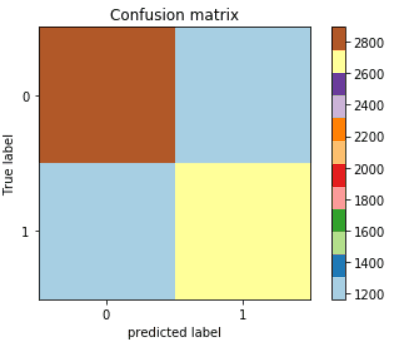
\includegraphics[width=12cm]{matrix.png}
\caption{Confusion Matrix} \label{fig:Confusion Matrix}
\end{figure}

Calculation can be a variety of evaluation indicators are as follows:
\begin{table}[h]
\centering
\caption{Evaluation Index}
\begin{tabular}{c|c}
\hline
acc & 0.691375\\
\hline
recall & 0.669119512814\\
\hline
precision & 0.693582325092\\
\hline
\end{tabular}
\label{tab2}
\end{table}]

As can be seen, relative to the previous logistic regression, the overall increase is larger. at this time,
The impact of a relatively small sample of bad clients has been greatly reduced. Will not appear always tend to
Evaluate as a good customer. It appears that over-sampling and under-sampling play a more significant role in the decision tree.
The common credit rating indicators available on the web show that 60\% is acceptable and 70\% is good.
\begin{figure}[h]
\small
\centering
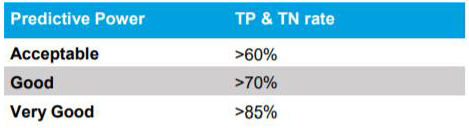
\includegraphics[width=12cm]{ei.png}
\caption{Matrix evaluation index} \label{fig:Matrix evaluation index}
\end{figure}

% \begin{Theorem} \label{thm:latex}
% \LaTeX
% \end{Theorem}
% \begin{Lemma} \label{thm:tex}
% \TeX .
% \end{Lemma}
% \begin{proof}
% The proof of theorem.
% \end{proof}

\begin{thebibliography}{99}
% \bibitem{1} D.~E. KNUTH   The \TeX{}book  the American
% Mathematical Society and Addison-Wesley
% Publishing Company , 1984-1986.
% \bibitem{2}Lamport, Leslie,  \LaTeX{}: `` A Document Preparation System '',
% Addison-Wesley Publishing Company, 1986.
\bibitem{1}\url{https://zhuanlan.zhihu.com/p/27770760}
\bibitem{2}\url{http://news.cnfol.com/guoneicaijing/20180124/25946369.shtml}
\bibitem{3}\url{https://en.wikipedia.org/wiki/Credit_scoret}
\bibitem{4}\url{https://zhuanlan.zhihu.com/p/30026040}
\bibitem{5}\url{https://help.aliyun.com/document_detail/55269.html?spm=5176.10695662.1996646101.searchclickresult.2b4af88cKoTF8e
}
\end{thebibliography}

\end{document}

%% 
%% This work consists of these files mcmthesis.dtx,
%%                                   figures/ and
%%                                   code/,
%% and the derived files             mcmthesis.cls,
%%                                   mcmthesis-demo.tex,
%%                                   README,
%%                                   LICENSE,
%%                                   mcmthesis.pdf and
%%                                   mcmthesis-demo.pdf.
%%
%% End of file `mcmthesis-demo.tex'.
